
\documentclass[border=0.125cm]{standalone}
\usepackage{tikz}
\usetikzlibrary{positioning}
\usepackage{ifthen}
\usetikzlibrary{matrix,arrows.meta,quotes,shadows,decorations.pathreplacing,positioning,fadings}
\usepackage{cfr-lm}
\usepackage{graphicx}


\colorlet{mewnol}{blue!75!cyan}%
\colorlet{allanol}{blue!50!black}%

\begin{document}
	
	\tikzset{%
		every neuron/.style={
			circle,
			draw,
			minimum size=1cm
		},
		pattern neuron/.style={
			circle,
			draw,
			minimum size=2cm
		},
		neuron missing/.style={
			draw=none, 
			scale=4,
			text height=0.333cm,
			execute at begin node=\color{black}$\dots$
		},
	}

	\begin{tikzpicture}
		\foreach \m/\l [count=\y] in {1,2,3,4,5,missing,6,7}
		{
			\ifthenelse{\equal{\m}{missing}}
			{
				\node[neuron missing] (input-missing) at (4.5-2*\y,0.5) {};
			}{
				\node[every neuron] (input-\m) at (4.5-2*\y,0) {};
			}
		}
	
		\foreach \m/\l [count=\y] in {1,2,3,missing,4,5,6}
		{
			\ifthenelse{\equal{\m}{missing}}
			{
				\node[neuron missing] (p-missing) at (5-2.5*\y,6.5) {};
			}{
				\node[pattern neuron] (p-\m) at (5-2.5*\y,6) {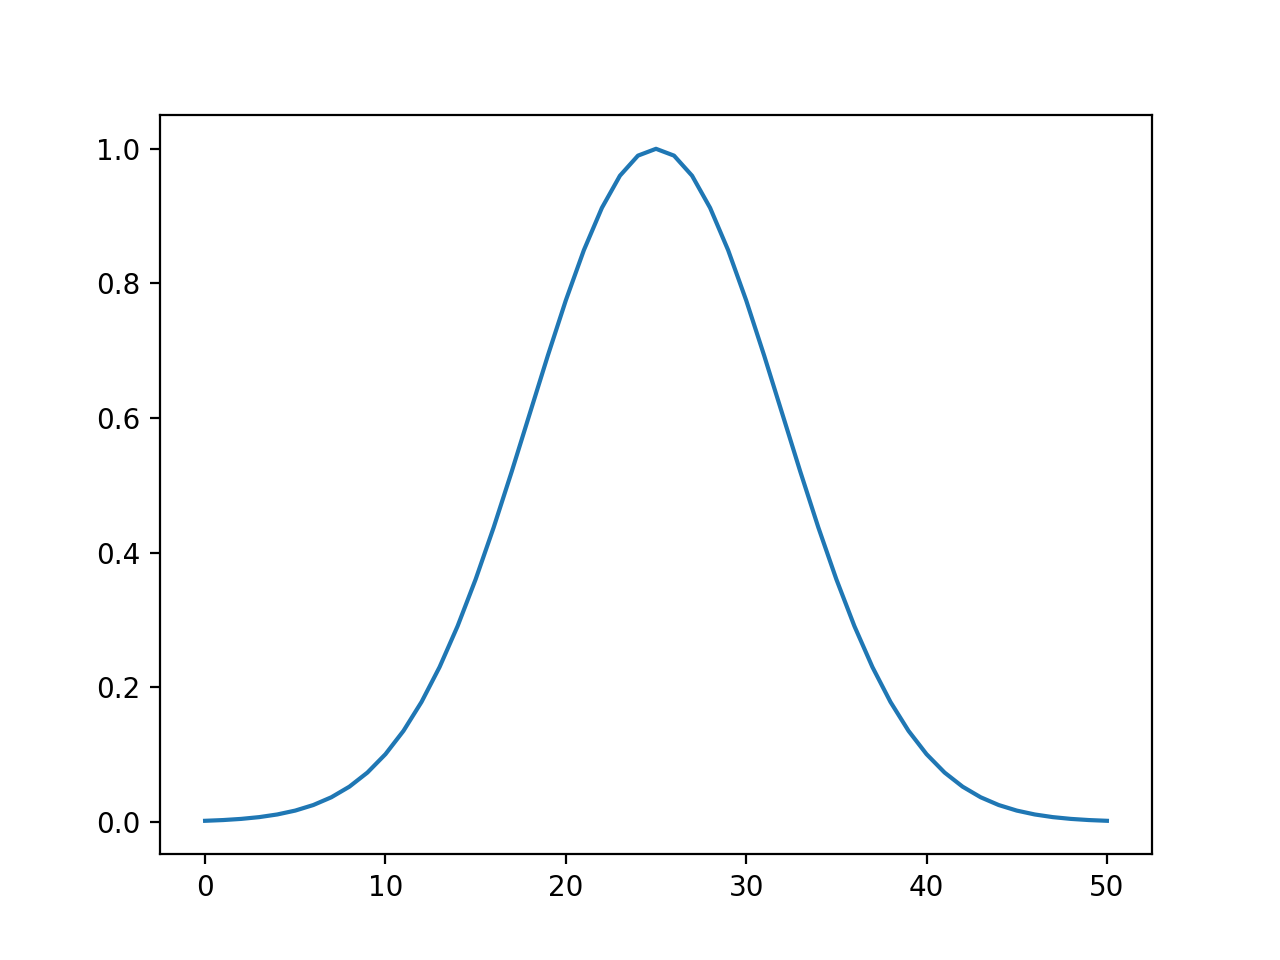
\includegraphics[width=.12\textwidth]{gaussian}};
			}
		}
	
		\foreach \m/\l [count=\y] in {1,2}
		{
			\ifthenelse{\equal{\m}{missing}}
			{
				\node[neuron missing] (out-missing) at (1.5-4*\y,12.5) {};
			}{
				\node[every neuron] (out-\m) at (1.5-4*\y,12) {};
			}
		}
		
		\foreach \m in {1,...,7}
			\foreach \n in {1,...,6}
				\draw[->] (input-\m) -- (p-\n);
		
		\draw[->] (p-1) -- (out-1);
		\draw[->] (p-2) -- (out-2);
		\draw[->] (p-3) -- (out-2);
		\draw[->] (p-4) -- (out-1);
		\draw[->] (p-5) -- (out-2);
		\draw[->] (p-6) -- (out-1);
		
		\node () at (6.5,0) {\textbf{Input units}};
		\node () at (6.5,6) {\textbf{Pattern units}};
		\node () at (6.5,12) {\textbf{Output units}};
	\end{tikzpicture}
\end{document}